\documentclass[a4paper, norsk, 12pt]{article}
\usepackage[utf8]{inputenc}   
\usepackage{graphicx} % Thingamajig for bilder
\usepackage{float} % Muliggjør strengere posisjonering av f.eks figurer og tabeller. Eks strengeste posisjonering \begin{figure}[H] 
\usepackage{parskip} % Enter enter gir mellomrom mellom paragrafer uten innrykk (indent / tab) 
\usepackage{verbatim} % Visning av tekst/kode/symboler/filer uten å bli lest som kode. Hvis du ønsker highlighted kode foreslår jeg \usepackage{minted} i stede!
\usepackage{csquotes} % Dependency reasons for babel, må stå før importen av babel!
\usepackage[norsk]{babel} % Gir tabeller og figurer norske navn, f.eks står det "Referanser" i stede for "References"
%\usepackage{array} 
\usepackage{booktabs} % For penere streker tror jeg
\usepackage[tableposition=top]{caption} % Fikser vspace for caption i tabeller
\usepackage{longtable} % For å lage laaaaaange tabeller
\usepackage{fancyhdr} % Fancy header 
\usepackage{hyperref} % Gir korrekt fremstilling av lenker eks: \url{https://www.overleaf.com} og gjør de klikkbare. Obs obs, plasseringen av denne pakken har noe å si!
\usepackage{amsmath} % Mattesymboler og funksjoner
\usepackage{changepage} % For å kunne bruke \adjustwidt for å la noe gå ut over de fastsatte margene

\usepackage{cancel} % Og denne for utstryking av to termer mot hverandre i en av ekvasjonene

% Kanskje verdt å putte surret mitt for tikz-figurene ett annet sted og laste det inn her for å gjøre det mer lesbart om man ikke er interessert i tikz?

\usepackage{tikz} %for tikz-figurer
\usetikzlibrary{arrows, decorations.markings}
\usetikzlibrary{decorations.pathreplacing, decorations.markings} % for spesielle piler i tikz-eksempel 2

% Arrow at middle of line
\tikzset{mid arrow/.style={postaction={decorate,decoration={ markings,
    mark=at position .5 with {\arrow[#1]{stealth}}
      }}},}

% Noen av mine favoritt-kommandoer å ha for hånden. Den STORE fordelen med å definere ting som dette er at med ett tastetrykk kan du endre hvordan noe ser ut i hele teksten. 

\newcommand{\Vect}{\mathcal{V}\textrm{ect}}
\newcommand{\C}{\ensuremath{\mathcal{C}}}
\newcommand{\ssg}{\scriptstyle}

\newcommand{\ie}{i.e.\:} % OBS: Grunnen til \: etter e.g. etc er for å unngå unaturlig lange mellomrom pga punktumet, men betyr at teksten som følger må skrives rett etter uten mellomrom :) 
\newcommand{\eg}{e.g.\:}
\newcommand{\st}{s.t.\:}
\newcommand{\cf}{c.f.\:}


% For siste tikz-bildet:
\def\Lcolor{red!10!black} 


% Definerer en ny kommando for tikz. [4] betyr at kommandoen tar inn 4 argument/tall, de er senere referert til som #1 = argument 1 etc. Det denne kommandoen gjør er å tegne en halvsirkel. (#1, #2)= origin, så #1 gir x-koordinater for midten av (halv)sirkelen, #2=y-koordinatet til midten. arc fra 180 grader til 0 grader = definert som (1,0) hvis man tegner sirkelen i R^2, og 180 blir da (-1,0) så du får øverste halvdel av sirkelen med radius #3. Den siste delen tegner en strek fra toppen av halvsirkelen til #4 lengde opp. 
\newcommand\drawMult[4]{
    \draw[thick] (#1, #2) arc(180:0:#3); 
    \draw[thick] (#1+#3, #2+#3)--(#1+#3, #2+#4);
}

\newcommand\drawDinat[5] {
    \filldraw[fill=green!40, draw=\Lcolor, thick](#1-#3,#2) -- (#1+#3,#2) -- (#1,#2-#4) -- cycle;
    \node [black,right=-1pt] at  (#1+#3,#2-#4/2)  {$ #5 $}; 
}

\newcommand\drawDinatE[5]{
    \drawMult{#1}{#2}{#3}{#4} 
    \drawDinat{#1+#3}{#2+1.2*#3}{0.6*#3}{0.6*#3}{#5}
}

\newcommand\drawOmega[3]{
    \filldraw[fill=white, draw=black, thick] (#1 , #2) rectangle (#1+#3, #2+0.4*#3); 
    \node[anchor=south] at (#1+0.5*#3, #2+0.4*#3) {\(\ssg \omega\)};
}

% Controls lar deg bøye linjer så de er nærmere controls-punktene (tenk deg at du klyper tak i linjen og drar den mot punktene som kommer etter controls + and, men linjen blir ikke nødvendigvis tvunget til å gå helt dit). Når man bruker disse må man nesten bare prøve seg litt fram for å se hva som ser bra ut til slutt. 

\newcommand\drawBraiding[4]{
    \draw[thick] (#1,#2).. controls (#1, #2+0.4*#4) and (#1+#3, #2+0.6*#4)..(#1+#3, #2+#4);
    \draw[thick] (#1+#3, #2).. controls (#1+#3, #2+0.1*#4) and (#1+0.7*#3, #2+0.3*#4).. (#1+0.6*#3, #2+0.4*#4);
    \draw[thick] (#1, #2+#4).. controls (#1, #2+0.9*#4) and (#1+0.4*#3, #2+0.6*#4).. (#1+0.4*#3, #2+0.6*#4); }

\newcommand\drawRightEval[3]{\draw[thick](#1, #2) arc(180:0:#3); \draw[thick, ->] (#1+#3, #2+#3)--(#1+#3-0.08, #2+#3); } % Tikz-definisjonene ble litt vel lange så puttet det i en egen fil

% \usepackage[acronym]{glossaries} % Pakke for å holde styr på akronymer, kan være grei ved større prosjekter.
%\usepackage[ddmmyyyy]{datetime}
% \usepackage{fontspec} % Lar oss bytte font

\usepackage[
  top=2cm,
  bottom=2cm,
%   left=2cm,
%   right=2cm,
  headheight=12pt,
  includehead,includefoot,
  heightrounded,
]{geometry} % Standard marger er for store imo, nå er de mindre.

% Bibliography management
%  see https://www.overleaf.com/learn/latex/Biblatex_citation_styles
%  and https://www.overleaf.com/learn/latex/Bibliography_management_in_LaTeX
% to use overleaf with reference manager
%  see: https://no.overleaf.com/blog/639-tip-of-the-week-overleaf-and-reference-managers
\usepackage[
    backend=biber, % Sets the backend to sort the bibliography, biber is the default one and recommended since it provides full localization for several commands and the styles for biber are easier to modify because they use standard LATEX macros.
    style=ieee % Sets the reference style
]{biblatex}
\addbibresource{referanser.bib} % Imports bibliography file


% Instillinger for fancyhdr 
\setlength{\headheight}{15.2pt}
\pagestyle{fancyplain}
\lhead{\fancyplain{}{Aleksander Karlsson}} % Tekst i venstre hjørne av header
\rhead{\fancyplain{}{This is a \textit{\textbf{fancy}} header}} % Tekst i høyre hjørne av header

\renewcommand{\arraystretch}{1.2} % Litt større mellomrom mellom hver rad i tabeller, standard er 1

\title{En ganske usaklig introduksjon til Overleaf og \LaTeX} % Tittel for hele dokumentet

\author{
    Aleksander M. Karlsson\\
    aleksander.mats.karlsson@gmail.com
} % Forfatter(e)
        
\date{Februar 2021} % Dato

%%%%%%%%%%%%%%%%%%%%%%%%%%%%%%%%%%%%%%%%%
%       Her begynner dokumentet         %
%%%%%%%%%%%%%%%%%%%%%%%%%%%%%%%%%%%%%%%%%
\begin{document}

    \maketitle % Genererer tittel, forfatter og dato
    % {\large \\Eilind Karlsson\\ Torjus Iveland\\ Maria Nylund \\}
    \newpage
    \tableofcontents % Genererer innholdsfortegnelse
    \pagenumbering{gobble} % Gobbles up the page numbering >:)
    
    \newpage % Sørger for at resten av innholdet starter på ny side.
    \pagenumbering{arabic} % Starter sidetall fra og med NÅ!
    
    \section{Introduksjon}
    Dette vokste plutselig til et litt større dokument enn jeg først tenkte. Ta en titt gjennom innholdsfortegnelsen/overskriftene og dropp å lese ting som ikke er relevant for deg og ditt.
    Hvis du har tilbakemeldinger eller spørsmål er det bare å ta kontakt!
    
    \subsection{Hva er \LaTeX?}
        Uttales lignende ``La-tek'' eller ``La-tech'' \underline{ikke} som gummistoffet kondomer er laget av. 
        \LaTeX{} er et sett med makroer for \TeX{} som gjør det lettere å skrive dokumenter. \LaTeX{} gir det deg standard makroer for mange funksjoner som f.eks seksjoner. Tenk på  \LaTeX{} som en mer brukervennlig utviding av \TeX.
        % TODO: Forklar hva det er
    
    \subsection{Hva er Overleaf?}
        Basically Google docs for \LaTeX. Samarbeid i sanntid. Null nedlasting, bare å lage konto og sette igang! 
        Dersom du ikke liker kompileringstiden er det fullstendig mulig å laste ned et lokalt program for å skrive \LaTeX.
        Dette er dog ikke dekket i denne guiden.
        
        \textit{PS: Hvis du er student hos NTNU legg til studentmailen din i kontoen så kan du søke om gratis Professional konto!\\
        PPS: Ha en privat email koblet til kontoen i tillegg så du ikke mister tilgang når du slutter på universitetet!\\
        PPPS: Hvorfor ikke koble til GitHub-kontoen din når du først er i gang?}
    
    \subsection{Hvorfor \LaTeX?}
        \LaTeX{} har en brattere læringskurve enn andre vanlige tekstbehandlingsprogrammer, men til gjengjeld får du fullstendig kontroll over resultatet. Dette gir (som oftest) et \textit{\textbf{S E  X Y}}, profesjonelt og ryddig resultat. Med det sagt så er ikke \LaTeX{} for alle, men hvor mange kjenner du som faktisk kan å bruke Word sikkerlig anyways?
        
        Kort sagt, har du forøkt å skrive matematiske formler i Word/Docs vil livet ditt bli bli lang lettere med \LaTeX!
        Om du bare ønsker denne funksjonaliteten finnes det programmer som lar deg gjøre om formler fra \LaTeX{} til andre programmer.
        
        \LaTeX{} er veldig populært i noen deler av akademia. Så mye som 97\% av artikler publisert innen mattematikk er skrevet i \LaTeX{}, og det er mange ressurser og formuer tilgjengelig for tips og hjelp!
        Det er også populært i felt som Statistikk (89\%), Fysikk (74\%) og Datateknologi (46\%) \cite{brischoux2009don}. For humaniora og andre fag er bruken mindre utbredt, og totalen bland de undersøkte feltene viste at rundt 27\% av alle publiserte artikler er skrevet i \LaTeX. 
    
%\section{Terminologi}
\section{Ting og tang i Overleaf}
    Her forsøkes det å definere forskjellige begreper og knapper som vil brukes videre i denne guiden.
    
    \subsection{Knapper og innstillinger i Overleaf}
        Det er to hovedområder i Overleaf. Til høyre er PDFen. Dette er det ``ferdige'' produktet \LaTeX{} genererer fra informasjonen til venstre. Til venstre er tekstområdet. Det er her man skriver teksten og kommandoene som vil vises i PDFen.
        
        \begin{figure}[h!]
            \centering
            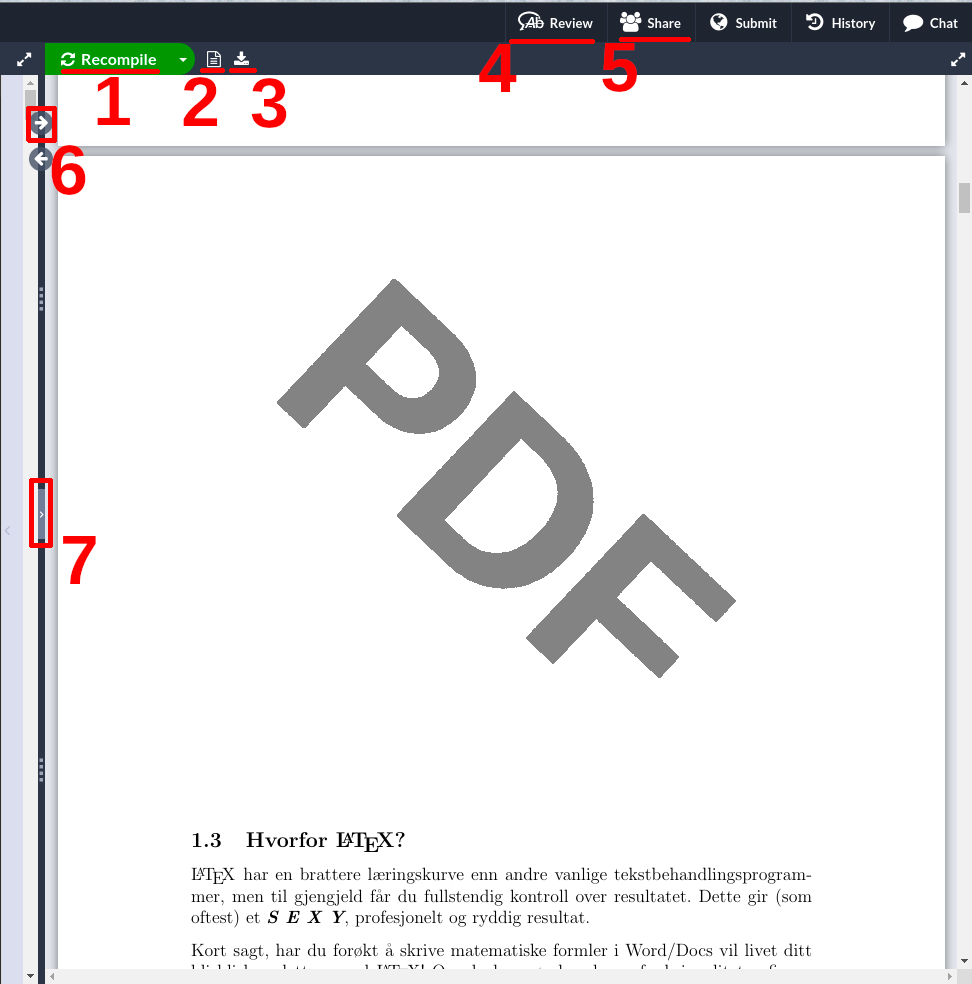
\includegraphics[width=\textwidth]{bilder/Latex-guide-pdf.png}
            \caption{Oversikt over PDF-området i et Overleaf-vindu}
            \label{fig:oversikt-overleaf-pdf}
        \end{figure}
    
        I figur \ref{fig:oversikt-overleaf-pdf} er det fremhevet et par viktige knapper i PDFen.
        \begin{enumerate}
            \item Recompile laster inn PDFen på nytt. Dvs alt som er gjort siden sist vil vises på PDF-en. Hvis du er i tekstområdet vil du også kunne klikke ctrl+s eller cmd+s for å rekompilere.
            \item Ved siden av recompile kan du klikke for å se på feilmeldinger. Dersom det vises et rødt tall her er det lurt å ta en titt. Mer om dette i seksjon \ref{sec:feilmeldinger}.
            \item Last ned PDF. Husk å recompile før du trykker på denne knappen for å få med alle endringer!
            \item Review åpner kommentarfeltet i tekstområdet, og lar deg se gjennom dine og andres kommentarer.
            \item Share lar deg dele prosjektet med andre, via link eller epost. Husk edit-link hvis de skal få skrive i dokumentet!
            \item $\rightarrow$ symbolet vil ta deg fra linjen du er på i tekstområdet til nogenlunde riktig sted i PDFen. Dette funker andre veien, bare dobbeltklikk i PDFen for å komme til nogenlunde riktig sted i tekstområdet.
            \item Denne knappen skjuler PDFen. Jeg bruker den sjeldent, men nå har du en pekepinn på hvorfor PDFen din plutselig forsvant!
        \end{enumerate}
        
            % \item main.tex er det standarde navnet for grunnfilen. Det er denne filen som \LaTeX{} leser når den skal lage PDFen. Ikke endre navnet dette navnet med mindre du vet hva du gjør.
            % \item Øverst til venstre er innstillinger for Overleaf, denne vises nærmere i figur \ref{fig:innstillinger-overleaf}. 
        % TODO: Legg til resizing av vinduer + kanskje mer fra overleaf sin side.
        
        
        \begin{figure}[H]
            \centering
            \includegraphics[width=\textwidth]{bilder/latex-guide-tekstområdet.png}
            \caption{Oversikt over tekstområdet i et Overleaf-vindu}
            \label{fig:oversikt-overleaf-tekstområdet}
        \end{figure} 
        
        I figur \ref{fig:oversikt-overleaf-tekstområdet} er det fremhevet et par viktige knapper i tekstområdet.
        \begin{enumerate}
            \item Menyen til Overleaf, mer om dette i figur \ref{fig:innstillinger-overleaf}.
            \item Tre knapper:
            \begin{enumerate}
                \item Lag ny fil: lag en ny fil i prosjektet. F.eks innhold.tex, eller referanser.bib.
                \item Ny mappe: Opprett mapper, f.eks bildemappe.
                \item Last opp: Last opp filer til prosjektet, f.eks bilder.
            \end{enumerate}
            \item Prosjektnavnet: Endrer kun navnet for hva prosjektet heter i Overleaf, ikke tittel e.l.
            \item Viser kommentarer. Samme funksjon som knapp 4 i figur \ref{fig:oversikt-overleaf-pdf}.
            \item Skjuler sidemenyen.
            \item main.tex, filen \LaTeX{} leser først.
        \end{enumerate}
    
    Hvis du trykker på knapp 4 i figur \ref{fig:oversikt-overleaf-tekstområdet} vil du få opp denne menyen. \textbf{Wordcount} teller antall ord som vises i PDFen, og \textbf{Spell Check} bør byttes til språket du skriver i så du slipper fryktelig mange røde streker i tekstområdet. Dette er ikke verdens beste stavekontroll, så ikke følg forslagene den kommer med slavisk, og les over før du leverer!
    \textbf{Compiler} er sjeldent nødvendig å endre, men i noen tilfeller kan det være nyttig. Hvis i tvil bruk standarden pdfLaTeX som kompilator!
    \textbf{Editor Theme} gir deg muligheten til å endre fargeskjemaet i tekstområdet. Er du et nattdyr vil du kanskje sette pris på et mørkere tema enn standarden.
    
    {\tiny PS: Her kan du også bytte til VIM hvis du vil minske sjansen for å finne en romantisk partner med ~69 \%}
    
    \begin{figure}[H]
        \centering
        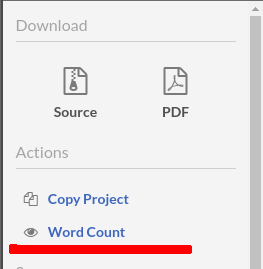
\includegraphics[width=.4\textwidth]{bilder/overleaf-2.png}
        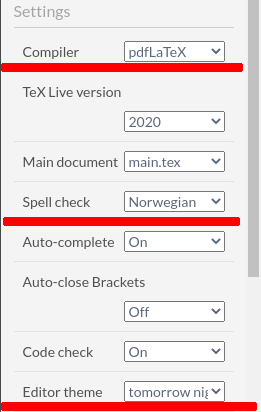
\includegraphics[width=.4\textwidth]{bilder/overleaf-3.png}
        \caption{Innstillinger i Overleaf}
        \label{fig:innstillinger-overleaf}
    \end{figure}
    
    \subsection{Andre funksjoner i Overleaf}
        Overleaf lar deg skrive kommentarer i tekstområdet, som du eller andre kan svare på eller løse. Marker litt tekst i tekstområdet og du vil få en ``add comment''-knapp i toppen høyre hjørne i tekstområdet. Kommentarfeltet kan også åpnet ved å klikke på ``Review''-knappen i høyre topp på siden. Ettersom du mest sannsynlig kun har en view-link (aka ikke redigeringsrettigheter) får du desverre ikke sett kommentarer i dette prosjektet.

        Overleaf hjelper deg å finne fram til riktig plass i både tekstområde/filstrukturen og PDFen.
        Du kan f.eks dobbeltklikke på denne teksten her i PDFen for å komme til både riktig fil og linje i tekstområdet. Dobbeltklikker du f.eks på tittelen i PDFen vil du komme til plassen tittelen genereres som er i main.tex filen. 
        
        For å gå fra en plass i tekstområdet til PDFen kan du klikke på ``$\longrightarrow$''-knappen som befinner seg litt under recompile-knappen.

        % Bytte til native pdf-viewer...

\section{Babys first project}
    Nå skal vi endelig lage et nytt prosjekt fra bunnen av.
    
    \subsection{Oppsett} 
        Gå til \url{https://www.overleaf.com/project} og klikk på ``New Project''.
        La oss gå for ``Blank project'' velg et navn så vi kan komme i gang!
        Vi begynner først med området over \textbackslash begin\{document\}.
        
        I tekstområdet blir du mest sannsynlig møtt noe \`a la:
        \verbatiminput{filer til innsetting/babys-first-doc}
        
        \vspace{3mm}
        Her kommer et forslag til endringer som bør gjøres med en gang:
        \verbatiminput{filer til innsetting/babys-improved-doc}
        
        Den første linjen definerer nå at dokumentet er av type artikkel, at sidene skal være på størrelse med et a4-ark, at fonten er 12pt stor (i motsetning til standard som er {\tiny 10pt}) og at vi skriver på norsk (hvis det er tilfellet).
        \textbackslash date\{\textbackslash today \} gir deg alltid dagens fulle dato hvis det er ønskelig.
        
        Anbefaler å faktisk opprette et prosjekt så du kan prøve ut ting videre i rapporten!
        
    \subsection{Min første paragraf}
        På tide å skrive litt. Først må vi bare gjennom en liten ting som VIL forvirre hvis du ikke vet det fra før.
        Så hvis du ser på tekstområdet til dette prosjektet vil du se en haug med backslasher ``\textbackslash''. Dette er leder-symbolet til \LaTeX!
        Hvis du bryter deg inn i leiligheten min og stjeler tastaturet mitt vil du finne backslash ved siden av tilbakeknappen.
        Nesten alt som står rett etter en backslash er en funksjon! Enten du vil eller ikke. 
        Dette er ikke det eneste symbolet som gir en litt annerledes funksjon enn å bare vises som symbolet. 
        
        Vil du skrive et prosenttegn i teksten din? Tough luck, det er nemlig symbolet for å ``kommentere ut'' altså skjule noe i tekstområdet slik at det ikke vises i PDFen. Hvis du dobbeltklikker her vil du se et eksempel på dette.
        %                             ░░░░░░░░░░░░░░░░░░░░░░█████████
        %                             ░░███████░░░░░░░░░░███▒▒▒▒▒▒▒▒███
        %                             ░░█▒▒▒▒▒▒█░░░░░░░███▒▒▒▒▒▒▒▒▒▒▒▒▒███
        %                             ░░░█▒▒▒▒▒▒█░░░░██▒▒▒▒▒▒▒▒▒▒▒▒▒▒▒▒▒▒▒██
        %                             ░░░░█▒▒▒▒▒█░░░██▒▒▒▒▒██▒▒▒▒▒▒██▒▒▒▒▒███
        %                             ░░░░░█▒▒▒█░░░█▒▒▒▒▒▒████▒▒▒▒████▒▒▒▒▒▒██
        %                             ░░░█████████████▒▒▒▒▒▒▒▒▒▒▒▒▒▒▒▒▒▒▒▒▒▒██
        %                             ░░░█▒▒▒▒▒▒▒▒▒▒▒▒█▒▒▒▒▒▒▒▒▒█▒▒▒▒▒▒▒▒▒▒▒██
        %                             ░██▒▒▒▒▒▒▒▒▒▒▒▒▒█▒▒▒██▒▒▒▒▒▒▒▒▒▒██▒▒▒▒██
        %                             ██▒▒▒███████████▒▒▒▒▒██▒▒▒▒▒▒▒▒██▒▒▒▒▒██
        %                             █▒▒▒▒▒▒▒▒▒▒▒▒▒▒▒█▒▒▒▒▒▒████████▒▒▒▒▒▒▒██
        %                             ██▒▒▒▒▒▒▒▒▒▒▒▒▒▒█▒▒▒▒▒▒▒▒▒▒▒▒▒▒▒▒▒▒▒▒██
        %                             ░█▒▒▒███████████▒▒▒▒▒▒▒▒▒▒▒▒▒▒▒▒▒▒▒██
        %                             ░██▒▒▒▒▒▒▒▒▒▒████▒▒▒▒▒▒▒▒▒▒▒▒▒▒▒▒▒█
        %                             ░░████████████░░░█████████████████
        %                          Great job! Du klarte å dobbeltklikke i PDFen!!!

        Men hvordan vise et prosenttegn i teksten spør du kanskje nå? Vel 100 \% av de som leser dette vil klare det!
        Essensielt putter du leder-symboet forran symbolet du vil vise. Så vil du se et prosenttegn i teksten vil du skrive backslash umiddelbart etterfulgt av prosenttegn ``\textbackslash\%''.
        Dette gjelder som sagt mange andre symboler som f.eks \$, \{, \}, \_ osv
        
    \subsection{Linjeskift}
        Den enkleste måten å skille to paragrafer fra hverandre er å klikke ``enter''-knappen to ganger, slik at det er minimum en tom linje mellom hver paragraf i tekstområdet. 
        Hvis du har åpnet et eget dokument og skriver to paragrafer vil standard linjeskift/separator mellom paragrafene være et innrykk (indent). Eks:
        {
            \setlength{\parindent}{2em} % Setter innrykk ved linjeskift kun inni denne blokken
            \parskip=0pt % Setter parskip til å ikke gjøre noe i denne blokken
            
            \subsubsection*{Eksempeltittel --- 3 paragrafer}
            Lorem ipsum dolor sit amet consectetur adipiscing elit quam varius orci, ridiculus mollis suspendisse arcu integer gravida fames nunc habitant. 
            
            Auctor rutrum aenean blandit dignissim tristique laoreet mi praesent taciti erat aptent, nascetur sagittis tortor himenaeos vestibulum bibendum montes lobortis ornare nec dis interdum, torquent fermentum congue diam class ultricies commodo hac netus maecenas. 
            
            Dictumst enim luctus habitant nunc auctor mus tellus ac dui ridiculus, inceptos ad est hendrerit feugiat torquent magna eu fringilla dis, nisi mauris fames quis vulputate hac massa platea orci.
        }
        
        Denne måten å skille mellom paragrafer har sine formål, men jeg syntes ofte det kan se litt klemt og uoversiktlig ut. For å endre dette pleier jeg å slenge inn \textbackslash usepackage\{parskip\} i main.tex (mellom \textbackslash documentclass[ ]\{\} og \textbackslash begin\{document\}). 
        
        \textit{PS: Om du ønsker å dele inn noe uten enter enter kan du skrive ledersymbolet to ganger på rad ``\textbackslash \textbackslash'' der du vil dele opp teksten.\\
        PPS: Om du ønsker å bruke standard linjeskift, men ønsker at en paragraf ikke skal ha innrykk kan du slenge inn \textbackslash noindent før paragrafen.}
        
\section{{\Huge Overskrifter}, {underoverskrifter} og {\tiny underunderoverskrifter}}
    Dette er oversikten over nivåene du kan dele inn teksten i:
    \verbatiminput{filer til innsetting/overskrifter}
    
    For dokumenttypen artikkel (aka det vi er i atm) er \textbackslash section\{ \} det øverste nivået! \textbackslash paragraph\{ \} og \textbackslash subparagraph\{ \} har jeg aldri hatt brukt, så har ingenting å si om dem tbh. 
    Hvis du ønsker å ikke ha nummererte seksjoner/overskrifter slik det er i denne guiden legger du til en stjerne før curlyboiene ``\{ \}''.
    Denne koden: 
    \begin{verbatim}
    \section*{Dette blir en overskrift uten tall}
        Helt vanlig tekst under overskriften.
        
        \subsection*{Underoverskrift uten tall}
            Helt vanlig tekst under underoverskriften.
            
            \subsubsection*{Underunderoverskrift uten tall}
                Helt vanlig tekst under underunderoverskriften.
    \end{verbatim}
    
    Vil se ut som dette \fbox{uten kantene rundt ofc}:
    \section*{\fbox{Dette blir en overskrift uten tall}}
        \fbox{Helt vanlig tekst under overskriften.}
        
        \subsection*{\fbox{Underoverskrift uten tall}}
            \fbox{Helt vanlig tekst under underoverskriften.}
            
            \subsubsection*{\fbox{Underunderoverskrift uten tall}}
                \fbox{Helt vanlig tekst under underunderoverskriften.}
    
    %For lange oppgaver 20+ sider (foreslår ikke å starte med \LaTeX for første gang på så lange oppgaver) kan det være verdt å vurdere dokumenttypen book e.l. Da får du f.eks brukt \textbackslash chapter osv. Dette gir dog noen endringer hvordan sidetall vises og andre ting så ta en titt på internett før du går den veien.
    
    \textit{PS: overskrifter uten tall vil ikke dukke opp i innholdsfortegnelsen!\\
    PPS: Det er ikke nødvendig å ``tabbe'' (flytte teksten innover) i det hele tatt, men jeg vil argumentere at det gjør koden lettere å lese/navigere.} 
    
\section{``Fnutter'', \textit{Italiensk} og Fet Tekst}
    
    \subsection{Sitater og fnutter/hermetegn}
        Tar du faget Tekstanalyse? Vil du bli \textbf{rosted} av und.ass? Hvis ja, ignorer dette!
    
        Den vanligste feilen er å bruke ``shift+2'' for å skrive dobbeltfnutt. Dette blir feil i PDFen, og den første dobbeltfnutten vil ikke vises. Hvis du mot formodning får den til å vises vil den uansett være feil vei! 
        
        Så, hvordan skrive `fnutter' og ``dobbeltfnutter'' riktig? 
        På mitt tastatur er startfnutten ``shift + knappen til venstre for tilbakeknappen'', og sluttfnutten er ``shift + stjerneknappen (*)''. Hvis du vil ha dobbeltfnutt trenger du to av disse symbolene før og etter det du vil ha inni. Ta en titt på tekstområdet for å se noen eksempler.
        
        \textit{PS: ``Shift+2'' fungerer som en slutt-dobbeltfnutt så du kan bruke den i stede for å klikke ``shift+stjerneknappen'' to ganger.}
        
    \subsection{\textit{Kursiv}}
        Dette er ingen kunst, putt \textbackslash textit\{tekst\} rundt teksten du vil ha i \textit{kursiv}. 
        \begin{verbatim}
    \textit{Denne teksten blir skakk}
        \end{verbatim}
        
        \textit{PS: Textit står for text italics, og emph (\textbackslash emph\{\}) betyr emphasis. De gir samme resultat i de fleste tilfeller, men avhengig av kontekst kan emph ha et annet utseende enn kursiv!}
        
    \subsection{Fet tekst}
        Trenger du et ord til å være modig, stikke ut litt fra resten av naboene? Da gjør du nesten det samme som for kursiv, bare plasser \textbackslash textbf\{tekst\} rundt teksten så blir den \textbf{P H A T}.
        \begin{verbatim}
    \textbf{Denne teksten blir fet}
        \end{verbatim}
        
        \textit{PS: `bf' står for bold face.} 
        
        
    \subsection{\texorpdfstring{\underline{Underlinje}}{Underlinje}}
        Som kursiv og fet tekst, bare med \textbackslash underline\{tekst\}. 
        \begin{verbatim}
    \underline{Denne teksten får underlinje}
        \end{verbatim}
        \underline{Denne teksten får underlinje}
        
    
        \textit{PS: \textbf{\underline{Å legge til flere effekter på en setning gjør den ikke lettlest}}}
\section{Lister}
    \subsection{Punktlister}
        Punk-lister er spesielt populære blant anarkister da de er uordnet.
        
        Her er en liste over sanne konspirasjoner vil sjokkere deg, uten noen spesiell rekkefølge selvsagt:
        \begin{itemize}
            \item Ronald Regan og Ronald Mc Donald er samme person
            \item[--] Mamma er en superhelt
            \item[$-$] Fugler er droner som spionerer på oss
            \item[$\ast$] Asterisk \& Obelix er en sann historie
        \end{itemize}
        
        Her er kilden til denne lista:
        \begin{verbatim}
    \begin{itemize}
        \item Ronald Regan og Ronald Mc Donald er samme person
        \item[--] Mamma er en superhelt
        \item[$-$] Fugler er droner som spionerer på oss
        \item[$\ast$] Asterisk \& Obelix er en sann historie
    \end{itemize}
        \end{verbatim}
        
        Hvis du vil kan du også nøste lister, altså putte en liste inni en liste inni en liste inni en liste inni en liste inni en liste inni en liste inni en liste, hvis du vil altså:
        \begin{itemize}
            \item En liste
            \begin{itemize}
                \item En liste inni en liste
                \begin{itemize}
                    \item En liste inni en liste inni en liste
                    \begin{itemize}
                        \item En liste inni en liste inni en liste inni en liste
                    \end{itemize}
                \end{itemize}
            \end{itemize}
        \end{itemize}
    
        Det svarte punktet er standard symbolet for punktlister, og for en liste inni en liste vil standarden være en strek.
        Hva som er standard symbol for et prosjekt kan også endres slik at du slipper å skrive det hver gang, men det kan du bruke din favoritt søkemotor til å finne ut av. Eller det må ikke være favoritten din, ingen tvinger deg.
        
    
    \subsection{Autoritære lister --- Tall og bokstaver}
        Så du er høyreekstrem og vil rangere elementene i lista di? 
        Her er en liste som gir deg grunner til at du er teit:
        \begin{enumerate}
            \item Tall er for nerder.
        \end{enumerate}
        
        Og her er kildekoden for denne lista:
        \begin{verbatim}
    \begin{enumerate}
        \item Tall er for nerder.
    \end{enumerate}
        \end{verbatim}
        
        Hvordan endre mellom tall, bokstaver eller romertall? Jeg søker det opp for hver gang men her er en grei link \url{https://www.latex-tutorial.com/tutorials/lists/}.
        Disse listene kan også nøstes.


\section{Importering av usepackages}
    Det er vanlig å ville ha flere funksjoner enn det som er standard innebygd i \LaTeX. Da må vi importere pakker! Vær litt varsom da noen pakker ikke fungerer sammen, og rekkefølgen kan ha noe å si. Dette er ikke et vanlig problem men noe å ha i bakhodet dersom det skulle oppstå problemer. Det er også lurt å vite hva en pakke gjør før vi legger den til. Jeg pleier å legge ved en kommentar som forklarer hva en pakke gjør for å gjøre det enklere for meg og andre å bruke funksjonene riktig. 
    % Tenker kanskje her siden det kommer en del imports etter hvert.


\section{Figurer} \label{sec:figurer}
    \subsection{Bilder} \label{sec:bilder}
        Lei av å sende dickpicks på snap? Sett det inn \LaTeX-dokumentet til gruppa di i stede!
        Begynn med å skrive \textbackslash begin\{figure\} + enter så vil du få noe sånt som dette:
        \begin{verbatim}
    \begin{figure}
        \centering
        \includegraphics{}
        \caption{Caption}
        \label{fig:my_label}
    \end{figure}
        \end{verbatim}
        Dette er et fint utgangspunkt, men hvis du setter inn bilder for første gang vil plasseringen og størrelsen kanskje være merkelig.
        
        \begin{figure}[H]
            \centering
            
\includegraphics{bilder/JavaScript4kidz.jpg}
            \caption{Dette ble litt vel stort}
            \label{fig:too_large_img}
        \end{figure}
        
        \begin{figure}[H]
            \centering
            
\includegraphics[width=.5\textwidth]{bilder/JavaScript4kidz.jpg}
            \caption{Dette var bedre}
            \label{fig:perfectly_normal_img}
        \end{figure}
        
        Hvordan ser dette ut i tekstområdet? Vel du kan ta en titt selv, men hvis du er for lat kommer figur \ref{fig:perfectly_normal_img} her:
        \begin{verbatim}
\begin{figure}[H]
    \centering 
    
\includegraphics[width=.5\textwidth]{bilder/JavaScript4kidz.jpg} 
    \caption{Dette var bedre}
    \label{fig:perfectly_normal_img}
\end{figure}
        \end{verbatim}
        
        [H] setter hvor streng \LaTeX{} skal være når det plasserer bildet. ``H'' er here (og \textbf{krever} \textbackslash usepackage\{float\}) Hvis du vil ha en mindre streng plassering/ikke lyst til å lese seksjonen om usepackages kan du prøve ``h'' eller ``h!''.
        
        \textbackslash centering midtstiller bildet i det horisontale planet.
        
        \textbackslash includegraphics setter faktisk inn bildet, hvis bilde ligger i en mappe (som her) må du gi hele lenken. Aka bilder + / + filnavnet + . + filtype $\rightarrow$ bilder/JavaScript4kidz.jpg.
        Det er også her vi kan sette størrelsen på bildet, i eksempelet er siden 0.5 (dvs 50 \%) av bredden til teksten, men du kan også skrive f.eks 10cm eller 15mm. 
        
        \textbackslash caption setter hva bildeteksten skal være. I oppgaver skal caption være under bilder, og skal forklare hva du ser på bildet!
        
        \textbackslash label gir deg noe å lenke til slik at du kan referere til bildet i teksten. Label må alltid komme etter caption i tekstområdet! Labelet skal også være unik slik at vi kan referere til bildet i teksten.
        
        \textbackslash ref\{fig:perfectly\_normal\_img\} vil gi tallet \ref{fig:perfectly_normal_img} ettersom dette er det \ref{fig:perfectly_normal_img} bildet. Dette endrer seg automatisk hvis du f.eks flytter bildet slik at det ikke er nr. \ref{fig:perfectly_normal_img} lenger.
        
        Blender bildet ditt inn i bakgrunnen? Sleng en \textbackslash fbox \{rundt \textbackslash includegraphics[]\{\}\} da vel:
        
        \begin{figure}[H]
            \centering 
            \fbox{
\includegraphics[width=2cm]{bilder/pixelated.PNG}}
            \caption{Her er det en fin ramme (fbox) rundt bildet}
            \label{fig:bordered_img}
        \end{figure}
        
        % Note: svg funker
        % Ved siden av hverandre
        
        
    \subsection{Tikz}
        Advarsel, dette er litt viderekommende greier! Ikke bruk tid her hvis det ikke er relevant/interessant! 
        
        Tikz er en fantastisk pakke som gjør det mulig å tegne kule figurer direkte i \LaTeX. Jeg er ikke veldig stødig på dette feltet men det kommer kanskje en litt mer utfyllende guide en gang i fremtiden. I mellomtiden kan du ta en titt på de kule tegningene jeg fikk fra søsterns bacheloroppgave i teoretisk kvantefeltsteori. 

        \begin{figure}[H]
            \centering
            \tikzset{every picture/.style={line width=0.75pt}} %set default line width to 0.75pt        
            \begin{tikzpicture}[x=0.75pt,y=0.75pt,yscale=-1,xscale=1]
                %uncomment if require: \path (0,300); %set diagram left start at 0, and has height of 300
                %Shape: Smiley Face [id:dp2033336285453986] 
                \draw   (291,150) .. controls (291,130.67) and (306.67,115) .. (326,115) .. controls (345.33,115) and (361,130.67) .. (361,150) .. controls (361,169.33) and (345.33,185) .. (326,185) .. controls (306.67,185) and (291,169.33) .. (291,150) -- cycle ; \draw   (310.6,138.1) .. controls (310.6,136.17) and (312.17,134.6) .. (314.1,134.6) .. controls (316.03,134.6) and (317.6,136.17) .. (317.6,138.1) .. controls (317.6,140.03) and (316.03,141.6) .. (314.1,141.6) .. controls (312.17,141.6) and (310.6,140.03) .. (310.6,138.1) -- cycle ; \draw   (334.4,138.1) .. controls (334.4,136.17) and (335.97,134.6) .. (337.9,134.6) .. controls (339.83,134.6) and (341.4,136.17) .. (341.4,138.1) .. controls (341.4,140.03) and (339.83,141.6) .. (337.9,141.6) .. controls (335.97,141.6) and (334.4,140.03) .. (334.4,138.1) -- cycle ; \draw   (308.5,164) .. controls (320.17,173.33) and (331.83,173.33) .. (343.5,164) ;
                %Curve Lines [id:da23991004776222824] 
                \draw    (274,344) .. controls (271,139.64) and (378,122.64) .. (374,344) ;
                %Curve Lines [id:da4778541646245862] 
                \draw    (539,169.61) .. controls (432,169.61) and (452,183.61) .. (413,115.64) .. controls (372,37.61) and (271,22.61) .. (227,139.61) .. controls (209.09,179.41) and (200.09,171.69) .. (93.61,170.62) ;
                \draw [shift={(92,170.61)}, rotate = 360.53] [color={rgb, 255:red, 0; green, 0; blue, 0 }  ][line width=0.75]    (10.93,-3.29) .. controls (6.95,-1.4) and (3.31,-0.3) .. (0,0) .. controls (3.31,0.3) and (6.95,1.4) .. (10.93,3.29)   ;
                
                % Text Node
                \draw (309,219) node [anchor=north west][inner sep=0.75pt]   [align=left] {Meg};
                % Text Node
                \draw (501,146) node [anchor=north west][inner sep=0.75pt]   [align=left] {Tikz};
            \end{tikzpicture}
            
            \caption[Meg og tikz]{
            Hvis dette også gjelder deg kan du eksportere tikz-kode fra Geogeobra (med litt varierende resultat) eller bruke det samme programmet jeg brukte her\protect\footnotemark.}
            \label{fig:tikz-is-hard}
        \end{figure}
        
        \footnotetext{\url{https://www.mathcha.io/editor}}
        
        % Trenger jo kanskje ikke forklare alt fordi det blir langt, men skader ikke å legge med noen eksempler på hva man kan gjøre med tikz uansett?
         
        %Disclaimer: vet dette ikke er ekstremt pent skrevet, tikz-figurene mine ble til litt underveis. Hadde jeg laget denne i dag hadde jeg feks gitt navn v1-v10 og skrevet en loop som tegner ut linjene for v_i-v_{i+1} etc. Hadde nok også laget en egen kommando for pilen midtveis så jeg ikke hadde trengt å skrive ut den linjen dobbelt. Men er vel rett fram å lese, og hvis de vil lære det er en bra måte å leke rundt med hva som forsvinner hvis de kommenterer ut forskjellige kommandoer for. Så har de noe å gå utifra i alle fall. 

        \begin{figure}[H]
            \centering     
            \resizebox{.7\linewidth}{!}{
                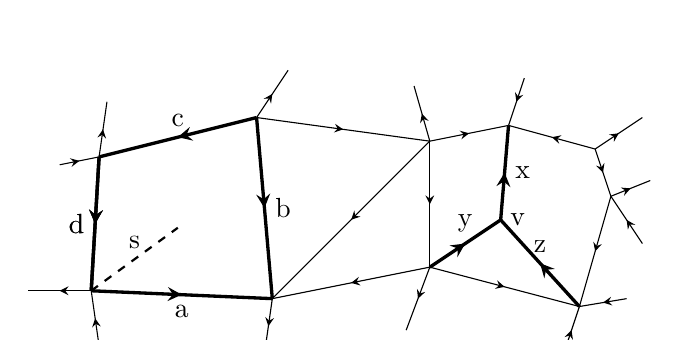
\begin{tikzpicture}
                    \coordinate (cd) at (-2.2, 1.8); 
                    \coordinate (bc) at (-0.2, 2.3);
                    \coordinate (ad) at (-2.3, 0.1);
                    \coordinate (ab) at (0,0);
                    %Draw face with abcd:
                    \draw[very thick, black, postaction={mid arrow=black}]  (bc) -- (cd) node[midway, above]{c};
                    \draw[very thick, black, postaction={mid arrow=black}]  (cd) -- (ad) node[midway, left]{d};
                    \draw[very thick, black, postaction={mid arrow=black}]  (ad) -- (ab) node[midway, below]{a};
                    \draw[very thick, black, postaction={mid arrow=black}]  (cd) -- (ad) node[midway, left]{d};
                    \draw[very thick, black, postaction={mid arrow=black}]  (bc) -- (ab) node[midway, right]{b};
                    \draw[dashed, thick, black] (ad)--(-1.2, 0.9) node [midway, above]{s};
                    %"Normal lattice" in the middle
                    \coordinate (v1) at (2, 2);
                    \coordinate (y) at (2, 0.4);
                    \draw[black, postaction={mid arrow=black}] (bc)--(v1);
                    \draw[black, postaction={mid arrow=black}] (v1)--(ab);
                    \draw[black, postaction={mid arrow=black}] (v1)--(y);
                    \draw[black, postaction={mid arrow=black}] (y)--(ab);
                    %Vertex with three edges
                    \coordinate (z) at (3.9, -0.1);
                    \coordinate (v) at (2.9, 1);
                    \coordinate (x) at (3, 2.2);
                    \coordinate (v2) at (4.1, 1.9);
                    \coordinate (v3) at (4.3, 1.3);
                    \draw[black, postaction={mid arrow=black}] (y)--(z);
                    \draw[black, very thick,  postaction={mid arrow=black}] (y)--(v) node[midway, above]{y};
                    \draw[black, very thick,  postaction={mid arrow=black}] (z)--(v) node[midway, above]{z};
                    \draw[black, very thick,  postaction={mid arrow=black}] (v)--(x) node[midway, right]{x};
                    \draw (v) node[right]{v};
                    \draw[black, postaction={mid arrow=black}] (v1)--(x);
                    \draw[black, postaction={mid arrow=black}] (v2)--(x);
                    \draw[black, postaction={mid arrow=black}] (v2)--(v3);
                    \draw[black, postaction={mid arrow=black}] (v3)--(z);
                    \draw[black, postaction={mid arrow=black}] (4.7, 0.7)--(v3);
                    \draw[black, postaction={mid arrow=black}] (v3)--(4.8, 1.5);
                    \draw[black, postaction={mid arrow=black}] (v2)--(4.7, 2.3);
                    \draw[black, postaction={mid arrow=black}] (3.2, 2.8)--(x);
                    \draw[black, postaction={mid arrow=black}] (v1)--(1.8, 2.7);
                    \draw[black, postaction={mid arrow=black}] (bc)--(0.2, 2.9);
                    \draw[black, postaction={mid arrow=black}] (cd)--(-2.1, 2.5);
                    \draw[black, postaction={mid arrow=black}] (-2.7, 1.7)--(cd);
                    \draw[black, postaction={mid arrow=black}] (ad)--(-3.1, 0.1);
                    \draw[black, postaction={mid arrow=black}] (-2.2, -0.6)--(ad);
                    \draw[black, postaction={mid arrow=black}] (ab)--(-0.1, -0.7);
                    \draw[black, postaction={mid arrow=black}] (y)--(1.7, -0.4);
                    \draw[black, postaction={mid arrow=black}] (3.7, -0.7)--(z);
                    \draw[black, postaction={mid arrow=black}] (4.5, 0)--(z);
                \end{tikzpicture}  
            }
            \caption{An illustration of a two-dimensional lattice with oriented edges. The thick lines show the support of a face operator on the left and a vertex operator on the right.}
            \label{fig:søs-tikz-1}
        \end{figure}


        \begin{figure}[H]
            \centering 
            \resizebox{.5\linewidth}{!}{
                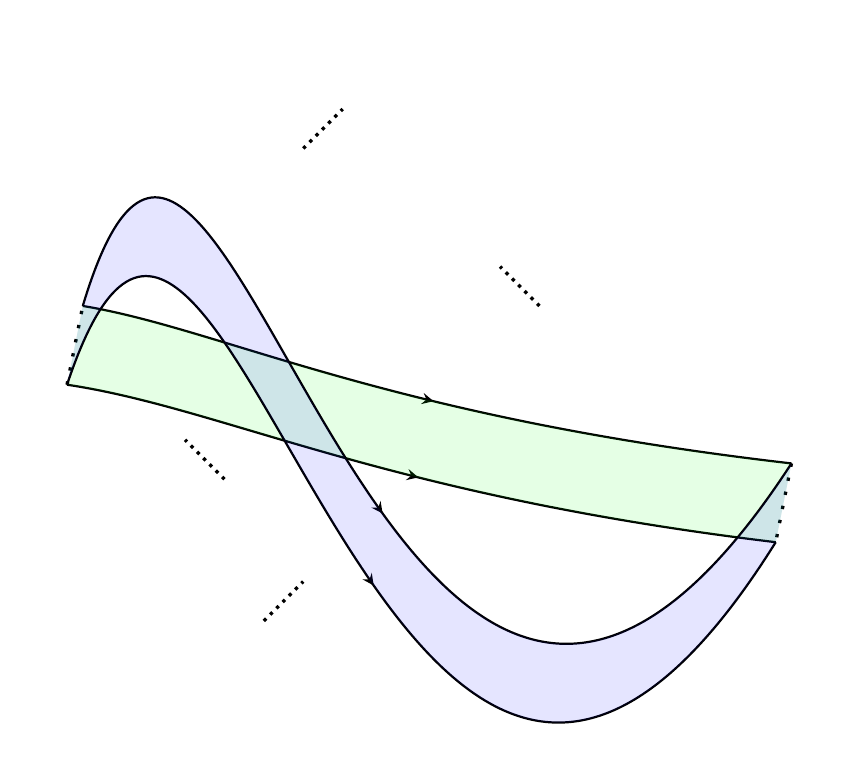
\begin{tikzpicture} 
                    \clip (-0.5,-5) rectangle (9.5,4);
                    %Define start and endpoints:
                    \coordinate (a) at (0,0);
                    \coordinate (b) at (0.2,1);
                    \coordinate (d) at (9,-2);
                    \coordinate (c) at (9.2, -1);
                    %Define arc a and b (enkel)
                    \def\arca{ (a) .. controls (2,-0.3) and (4,-1.4) .. (d)}
                    \def\arcb{ (b) .. controls (2, 0.7) and (4, -0.4) .. (c)}
                    \def\arcbinv { (c) .. controls (4, -0.4) and (2, 0.7) .. (b) }
                    %Draw everything with arc a and arc b (enkel) - green:
                        \draw[black, thick,  postaction={mid arrow=black}] \arca ;
                        \draw[black, thick,  postaction={mid arrow=black}] \arcb ;
                        \draw[black, very thick, loosely dotted] (a) -- (b);
                        \draw[black, very thick, loosely dotted] (c) -- (d);
                        \path[fill=green, opacity=0.1] (a) -- \arca -- (d) -- (c) -- \arcbinv -- (b)--cycle;
                    %Define and draw fancy (more extreme ribbon) - blue:
                    \def\arcc { (a).. controls (2, 6) and (4, -10) ..(d)}
                    \def\arcd { (b) .. controls (2,7) and (4,-9) .. (c) }
                    \def\arcdinv { (c) .. controls (4,-9) and (2,7) .. (b)}
                        \draw[black, thick,  postaction={mid arrow=black}] \arcc ;
                        \draw[black, thick,  postaction={mid arrow=black}] \arcd ;
                        \path[fill=blue, opacity=0.1] (a) -- \arcc --(d) --(c) -- \arcdinv --(b) --(a) --cycle;
                    %Excitations randomly placed around:
                        \draw[black, very thick, dotted] (3, 3)--(3.5,  3.5);
                        \draw[black, very thick, dotted] (6, 1)--(5.5, 1.5);
                        \draw[black, very thick, dotted] (2, -1.2)--(1.5, -0.7);
                        \draw[black, very thick, dotted] (2.5, -3)--(3, -2.5);
                \end{tikzpicture}   
            }
            \caption[Dette er en kort alternativ figurtekst]{An illustration of how a ribbon can be deformed into another one without crossing any excitation, here displayed as dotted lines. Hence, the ribbon operators corresponding to both ribbons will act in exactly the same way.}
            \label{søs-tikz-2}
        \end{figure}
        
        \def\width{0.7}
        \def\height{0.7}
        \def\shift{-5.8*\width} %forhåndsdefinerte lengder, hvis jeg vil ha figuren større/høyere etc så kan jeg bare endre på størrelsen her. Veldig praktisk å lage figurer med forhåndsdefinerte lengder for å kunne endre på dem uten å måtte redigere alle tall (som i mine figurer over)
        
        %Note: mange forhåndsdefinerte kommandoer i denne figuren, de kan finnes i main.tex før starten av dokumentet. Igjen veldig praktisk å forhåndsdefinere ting som man tegner/illustrerer ofte så går det mye fortere!

        \begin{figure}[H]
            \centering
            \begin{tikzpicture}
                \draw[thick](\shift+0.5*\width, 0.5*\height).. controls (\shift+0.5*\width, 0.8*\height) and  (\shift+1.1*\width, 1.5*\height).. (\shift+1.1*\width, 2*\height);
                \draw[thick](\shift+2.5*\width, 0.5*\height).. controls(\shift+2.5*\width, 0.8*\height) and (\shift+1.9*\width, 1.5*\height).. (\shift+1.9*\width, 2*\height);
                \drawDinatE{\shift}{0}{0.5*\width}{0.5*\height}{\ssg \iota^L_x}
                \drawDinatE{\shift+2*\width}{0}{0.5*\width}{0.5*\height}{\ssg \iota^L_y}
                \drawOmega{\shift+0.9*\width}{2*\height}{1.2*\width}
                \node[anchor=north] at (\shift, 0) {\(\ssg x^\vee \)};
                \node[anchor=north] at (\shift+\width, 0) {\(\ssg x^{\phantom\vee} \)};
                \node[anchor=north] at (\shift+2*\width, 0) {\(\ssg y^{\vee} \)};
                \node[anchor=north] at (\shift+3*\width, 0) {\(\ssg y^{\phantom\vee} \)};
            %%%
                \node at (-1.5*\width, \height){:=};
            %%%
                \drawBraiding{\width}{0}{\width}{\height}
                \drawBraiding{\width}{\height}{\width}{\height}
                \node[anchor=north] at (\width, 0){\(\ssg x^{\phantom\vee}\)};
                \node[anchor=north] at (2*\width, 0){\(\ssg y^{\vee}\)};
                \drawRightEval{0}{2*\height}{0.5*\width}
                \drawRightEval{2*\width}{2*\height}{0.5*\width}
                \draw[thick](0, 2*\height)--(0, 0) node[anchor=north]{\(\ssg x^\vee\)};
                \draw[thick](3*\width, 2*\height)--(3*\width, 0) node[anchor=north]{\(\ssg y^{\phantom\vee}\)};
            \end{tikzpicture}   
            \caption{The Hopf pairing \(\omega\)}
            \label{søs-tikz-3}
        \end{figure}



    \subsection{Matplotlib}
        % TODO: Sett inn IR grafen her?
        Under construction
    \subsection{Grafer}
        % TODO: Sett inn npl grafene her?
        Under construction
    

\section{Tabeller}
    Hvis du ikke har lyst til å lage egne tabeller fra bunnen av finnes det flere webbaserte verktøy du kan ta i bruk, f.eks \url{https://www.tablesgenerator.com/}.
    
    \subsection{Enkle tabeller}
    
        La oss starte med en enkel tabell. Vi begynner med å skrive \textbackslash begin\{table\} og klikker enter. Da vil du få noe som ligner litt på dette:
        
        
        \begin{verbatim}
\begin{table}[H]             % H er igjen plassering av tabellen 
    \caption{``bildetekst''} % Skal plasseres over \begin{tabular}
    \label{tab:keybinds}     % nå skal det stå tab:+unik identifikator
    \centering               % midtstiller tabellen
    \begin{tabular}{cc}      % begynner tabellen, cc betyr at det vil 
                             være to kolonner med sentrert tekst
        Key & Description \\ % Her kommer radene, de er delt opp 
                             med `&' tegn innad i radene, 
                             og `\\' for å skille mellom rader
        \hline\hline         % \hline gir horisontale linjer, 
                             så dette gir to horisontale linjer
        W & Move inwards \\
        S & Move outwards \\
        A & Move to the left \\
        D & Move to the right \\\hline
    \end{tabular}
\end{table}
        \end{verbatim}
        Dette resulterer i denne tabellen:
        \begin{table}[H]
            \caption{I tabeller skal denne ``bildeteksten'' være \textbf{OVER} tabellen!}
            \label{tab:keybinds}
            \centering
            \begin{tabular}{cc}
                Key & Description \\
                \hline\hline
                W & Move inwards \\
                S & Move outwards \\
                A & Move to the left \\
                D & Move to the right \\\hline
            \end{tabular}
        \end{table}
        
        Som nevnt i figurteksten skal altså typisk sett \textbackslash caption befinne seg over tabeller. Hovedgrunnen til dette er at tabeller ofte kan bli lange og du vil derfor forklare hva som kommer! Av diverse grunner er ikke dette standarden i \LaTeX, og det holder ikke kun å flytte captionen opp over \textbackslash begin\{table\}. Den blir plassert for nærme tabellen, spesifikt 10pt (ca 3.5 mm) for nærme. En enkel fiks er å enten legge til en \textbackslash vspace\{10pt\} til slutt inni captionen. Dette er ikke en elegant løsning, så her kan pakken ``caption'' foreslåes da de fikser dette mellomrommet automatisk. 
        
        Sleng inn denne i main.tex og flytt så caption over tabellen så blir mellomrommet korrekt! Det er hvertfall det jeg har gjort i dette dokumentet!
        \begin{verbatim}
    \usepackage[tableposition=top]{caption}
        \end{verbatim}
        
        Når det er unnagjort kan vi begynne med hvordan man faktisk endrer på formateringen og innholdet av tabellen. Linjen:
        \begin{verbatim}
    \begin{tabular}{cc}      
        \end{verbatim}
        Definerer både hvor mange kolonner det skal være, og hvordan de skal se ut. I dette tilfellet er det ``cc'' i den siste blokken. Dette betyr at vi får to kolonner, med sentrert (c for centered) tekst. Disse `c'-ene kan byttes ut med mye rart, men de mest vanlige alternativene er c, l og r for centered, left- og right-adjusted tekst. Det er også her du legger inn vertikale linjer hvis du vil ha det. F.eks vil
        \begin{verbatim}
    \begin{tabular}{|c|c|c|}
        \end{verbatim}
        Resultere i tre kolonner med sentrert tekst, hvor det er vertikale linjer både utenfor og mellom hver av kolonnene. 
        
        Når kolonnene er definert kan vi begynne å fylle inn radene:
        \begin{verbatim}
    Key & Description \\\hline
    W & Move inwards \\
    S & Move outwards \\
        \end{verbatim}
        Her ser dere tre rader med to kolonner. Det er \&-tegnet som skiller hvilken kolonne noe tillhører, dvs ``Key'' hører til kolonne 1, mens ``Description'' vil havne i kolonne 2. Antallet \&-tegn her må samsvare med antallet kolonner du har definert (antall \&-tegn i hver rad = antallet kolonner minus 1). Hver rad er skilt med ``\\''. Hvis du ønsker å ha horisontale linjer i tabellen legger du en ``\textbackslash hline'' mellom radene du ønsker å dele opp.
    
    
    \begin{table}[H]
        \minipage{0.3\textwidth}
            \centering
            \caption{sentrert tekst med kanter og linjer}
            \label{tab:center-tabell}
            \begin{tabular}{|c|c|c|c|}
                \hline
                \textbf{\#}  & \textbf{X}     & \textbf{Y}     \\\hline
                a   & 0.5   & 42    \\\hline
                b   & 0     & YEET  \\\hline
                c   & 190.5 & LEET  \\\hline
            \end{tabular}
        \endminipage\hfill
        \minipage{0.3\textwidth}
            \centering
            \caption{høyrestilt tekst uten kanter, en linje}
            \label{tab:høyre-tabell}
            \begin{tabular}{rrr}
                    & X     & Y     \\\hline
                a   & 0.5   & 12    \\
                b   & 0     & 82    \\
                c   & 190.5 & 1.02  
            \end{tabular}
        \endminipage\hfill
        \minipage{0.3\textwidth}
            \centering
            \caption{venstrestilt tabell med et par linjer}
            \label{tab:venstre-tabell}
            \begin{tabular}{l|llll}
                    & \multicolumn{2}{c}{X} & \multicolumn{2}{c}{Y}     \\\hline
                a   & 0.5   & 12 & 0.5   & 12   \\
                b   & 0     & 82 & 0.5   & 12   \\
                c   & 190.5 & 1.02  & 0.5   & 12
            \end{tabular}
        \endminipage\hfill
    \end{table}

    Her ser vi et par små tabeller med litt forskjellige stiler. Om teksten skal være sentrert, venstre- eller høyrestilt kommer an på typen og langden på innholdet. Dette kan være uavhengig fra kolonne til kolonne. Bruk det som passer best for innholdet!
    
    % \textit{PS: Vil du lage stilrene og sexy tabeller? Da dropper du vertikale linjer!}
    \textit{PS: Vil du lage lettleste, sexy og stilrene tabeller? Da vil jeg argumentere for å droppe vertikale linjer! Mellomrom (whitespace) mellom kolonnene ser mye bedre ut og fører sjeldent til et mindre leselig resultat. Sjekk ut \textbackslash arraystretch hvis du vil ha mer mellomrom\footnote{\protect\url{https://www.overleaf.com/learn/latex/Questions/How_do_I_change_column_or_row_separation_in_LaTeX_tables\%3F}}. Du kan også ta en titt i fila abolish-vertical-lines.tex i dette prosjektet (husk å rekompiler) for å se flere eksempler på tabeller med og uten vertikale linjer!}


    \subsection{Looooooongtable}
        Har du lyst til å lage en longboi? Tar den mer plass enn det er på en side? Da er longtable noe for deg. Men gidder jeg forklare det? Nopp. Finn det ut selv eller spør om hjelp.

        
    % \subsection{Makecell}
    % \subsection{tabularx, tabu, booktabs}
    
    
\section{Table of Contents}
    Tik ToC it's Table of Contents o'clock.
    \subsection{Overskrifter}
        Den vanligste formen for innholdsfortegnelse. \textbackslash tableofcontents genererer innholdsfortegnelsen for deg fra alle nummererte sections, sub- og subsub-sections. Denne linjen finner du som regel i main.tex rett etter \textbackslash begin\{document\} og \textbackslash maketitle. 
        
        \textit{PS: Elementene i innholdsfortegnelsen er hyperlenker som tar deg til riktig sted i PDFen hvis du klikker på de.\\
        PPS: Denne funksjonaliteten blir bevart av de fleste programmer selv om du laster ned PDFen.}
        
        \begin{verbatim}
    \tableofcontents % Genererer innholdsfortegnelse
    \newpage % Sørger for at følgende innhold starter på ny side
        \end{verbatim}
        
        Det er ikke uvanlig å slenge inn en \textbackslash newpage etter \textbackslash maketitle og \textbackslash tableofcontents for å sikre at de starter på en ny side.
        
    \subsection{Figurer}
        Det er også mulig å få en liste over figurer med \textbackslash listoffigures 
        \listoffigures
         
        I figur \ref{fig:søs-tikz-1} er figurteksten kanskje litt i lengste laget. Dette kan fikses ved å skrive en alternativ figurtekst til bildet slik jeg har gjort i figur \ref{søs-tikz-2}.
        Et eksempel på hvordan man gjør dette:
        \begin{verbatim}
\caption[Dette er alternativ]{Dette er en litt for lang figurtekst...}
        \end{verbatim}
        
    \subsection{Tabeller}
        Det er også mulig å få en liste over figurer med \textbackslash listoftables
        \listoftables 
        

\section{Referere, sitere og kilder}
    \subsection{Referer til noe fra teksten}
        Figurer og tabeller skal helst ha et label. Dette gjør at vi kan referere til disse ved å skrive textbackslash ref\{ det som står i labelet her \}:
        \begin{verbatim}
    Dette er tekst som viser til figur \ref{fig:bordered_img}.
        \end{verbatim}
        Resultatet:
        
        Dette er tekst som viser til figur \ref{fig:bordered_img}.
        
        \autoref{fig:bordered_img}
        
        Her kan du også se at tallet i PDFen er klikkbar, og tar deg til den korrekte figuren. Denne funksjonaliteten fungerer også med formler, tabeller, overskrifter, underoverskrifter, osv. Ønsker jeg å referere til overskriften ``Figurer'' må også denne overskriften ha et label:
        \begin{verbatim}
    \section{Figurer} \label{sec:figurer}
        \subsection{Bilder} \label{sec:bilder}
        \end{verbatim}
        
        Nå kan vi også referere i teksten til denne overskriften:
        
        I avsnitt \ref{sec:figurer} vil du finne figurer. Informasjon om bilder finner du i \ref{sec:bilder}.\\
        
        Hvis du ønsker å referere til sidetallet er også dette mulig med \textbackslash pageref.
        \begin{verbatim}
    På side \pageref{sec:bilder} finner du mer info om bilder.
        \end{verbatim}
        Resultat:
        
        På side \pageref{sec:bilder} finner du mer info om bilder.
            
        % https://www.bibme.org/mla/journal-citation
    \subsection{Lage kilder}
        Har du en bok, artikkel, studie, etc du ønsker å vise til? Da må vi først sette opp et verktøy for å håndtere kilder! Jeg pleier å bruke biblatex for dette.
        
        Vi starter med å legge til et par linjer i main.tex:
        \begin{verbatim}
    \usepackage[
        backend=biber, % Sets the backend to sort the bibliography, 
            biber is the default one and recommended since it provides full 
            localization for several commands and the styles for biber are 
            easier to modify because they use standard LATEX macros.
        style=ieee % Sets the reference style
    ]{biblatex}
    
    \addbibresource{referanser.bib} % Imports bibliography file        
        \end{verbatim}
        
        Her importeres pakken biblatex med et par parametere (valg). Det første valget ``backend = biber'' trenger du ikke tenke så mye over, la det stå for nå, så kan du heller sjekke ut andre alternativer på egenhånd. Det du derimot bør tenke over er hvilken stil du skal bruke. Her er style = ieee, og vil si at alle siteringer vil følge denne stilen. Andre vanlige alternativer kan du finne på Overleaf sin wiki\footnote{\protect\url{https://www.overleaf.com/learn/latex/Biblatex_citation_styles}}.
        Det er også mulig å definere hvilken rekkefølge kildene skal være sortert etter, merk at mange stiler stiller krav til hvilken sortering som skal brukes.
        
        Til venstre for tekstområdet finner du oversikten over filer. I dette prosjetet finnes det allerede en fil som heter ``referanser.bib'', men denne må du lage selv hvis du skal ha kilder. Denne filen skal inneholde alle kildene du vil bruke (mer om dette etterpå).
        Linjen \textbackslash addbibresource\{filnavn.bib\} legger til filen ``referanser.bib'' til main.tex slik at biblatex har noe å jobbe med. Du kan selfølgelig kalle denne filen hva du vil så lenge den slutter med ``.bib''.
        
        I dette dokumentet er referanse.bib filen allerede populert med et par kilder, og de kan se litt kompliserte ut. Men ta det med ro, du trenger ikke skrive disse for hånd! De fleste seriøse journaler har allerede ferdiglaget biblatex kilder. F.eks her \url{https://ieeexplore.ieee.org/abstract/document/8489629} vil du kanskje legge merke til ``Cite this''-knappen. Trykker du på knappen vil du kunne velge ``BibLaTeX''. Kopier dette over i referanse.bib filen så er du klar til å sitere denne artikkelen! På andre sider står det ikke nødvendigvis ``Cite this'', men kanskje noe som ``Export Bibtex Citation'' e.l. Dette er definitivt den mest korrekte siteringen du vil finne, men fortvil ikke dersom journalen din ikke har / du finner dette. Da kan du bruke f.eks \url{https://www.bibme.org/bibtex/website-citation} for å søke på url, ISBN, tittel og forfatter for å generere en kilde på bibtex format. 
        
        Den eneste endringen jeg foreslår å gjøre her er den første linjen av hver kilde:
        \begin{verbatim}
    fra dette
    @article{8489629,
    til dette
    @article{beskrivelse-av-artikkelen,
        \end{verbatim}
        
        Dette er ``kallenavnet'' til kilden og fungerer veldig likt som label. Du må ikke gjøre dette, men det som står der er det du kommer til å skrive i tekstfeltet for å referere til kilden, så det er greit om du kaller kilden for noe du kommer til å kjenne igjen.
        
        Til slutt må vi ha med \textbackslash printbibliography der du vil vise kildelisten, her har jeg satt den mot slutten av main.tex (hvis du har vedlegg er det vanlig å ha det før vedlegget).
        
        \begin{verbatim}
    \newpage
    \printbibliography % Genererer og viser referanselisten 
                         (samt overskriften Referanser)
    \end{document} % Slutten av dokumentet
        \end{verbatim}
        
        
    \subsection{Sitere til andres arbeid}
        Nå skal du ha en kilde eller to å referere til! På tide å få det inn i teksten. Dersom alt er satt opp korrekt.
        
        Det finnes mange standarder og stiler for å gjøre dette, og jeg vil anbefale å lese gjennom reglene for den referansestilen du ønsker å bruke! F.eks i stilen IEEE (som brukes i dette dokumentet) skal det være et mellomrom mellom teksten og sitat-symbolet (dunno hva jeg skal kalle det, men det ser ut som ``[1]'' i IEEE). 
        
        Et eksempel på riktig bruk av sitering i IEEE:
        
        You Only Look Once (YOLO) is a cool and viable real-time image recognition approach \cite{DBLP:yolo9000}. 
        
        Vanlig feil for IEEE er å ikke ha mellomrom mellom ``approach'' og ``\cite{DBLP:yolo9000}'':\\
        You Only Look Once (YOLO) is a cool and viable real-time image recognition approach\cite{DBLP:yolo9000}.
        
        \begin{verbatim}
        Feil:
        approach\cite{DBLP:yolo9000}. 
        
        Riktig:
        approach \cite{DBLP:yolo9000}. 
        \end{verbatim}
        
        Her er det altså \textbackslash cite som gjør jobben. Det er også mulig å bruke \textbackslash parencite for å få parenteser rundt referansen (ikke relevant for denne stilen), eller \textbackslash footcite for å få referansen i fotnotene i stede.
        
        
    \subsection{Fotnoter}
        Fotnoter finner du her\footnote{``\textbackslash footnote\{ Dette dukker opp i fotnoten \}''}.
        
        

\section{Prosjekt- og mappestruktur}
    \subsection{Indentation}
        Som nevnt tidligere er jeg en forkjemper for å bruke innrykk i tekstområdet. Har du hatt ITGK (Python) bør dette virke kjent. Essensielt koker argumentet mitt ned til at det gjør tekstområdet penere, lettere å finne fram i og gjør det lettere å finne feil. Den eneste bekostningen er at du må klikke ``tab'' et par ganger.
        
    \subsection{Mapper og filnavn}
        Dette prosjektet er ikke så fryktelig stort, og krever ikke god mappestruktur. Det er fortsatt lurt å gjøre det til en vane slik at det er lettere for deg og andre å navigere filene. Bilde-mappen er ganske grei å ha hvis du skal sette inn bilder.
        
        Når det kommer til filnavn er det ikke så viktig hva de heter, bare sørg for at det er hensiktsmessige navn. Et tips hvis du vil ha en spesiell rekkefølge på filene er å navngi dem med tall slik som dette:
        
        1-Introduksjon.tex\\
        2-Diskusjon.tex\\
        3-Konklusjon.tex\\
        
        Hvis du deler opp i filer slik som dette må du sette inn filene i main.tex. Dette gjøres ved \textbackslash input\{1-Introduksjon\}. I mainfila i dette prosjektet ser du eksempler på dette.
        
    
\section{Matte}
    \subsection{amsmath og andre pakker her}
        %LOL, hvis dere er så nerdete at dere tar matte finner dere ut av dette selv!
        % Må flexe litt fancy formler da. bare så dere ser hvor sexy det ser ut


        Veldig verdt å vite når man skriver formler er at og-tegnet gir deg ting som er under hverandre, så i eksempelet under kommer =-tegnene rett under hverandre og sørger for at det ser ryddig ut. 

        Note: har også kommandoen \textbackslash Big for ekstra store paranteser (men kan brukes før andre ting også) for å gjøre ligninger med flere paranteser e.l. mer lesbare. Funker helt likt med andre størrelser (google it). Kan også bruke den mer dynamiske løsningen med left og right, som her \(F = G \left(  \frac{m_1 m_2}{r^2} \right)\). Viktig at både left og right skrives ut, ellers blir \LaTeX{} sur!

        \footnotesize %for at hele ligningen skal få plass gjør jeg skriften litt mindre. 
        \begin{adjustwidth}{-4cm}{-4cm}
            \centering
            \begin{align*}
                z\frac{d}{dz} \hat{\Phi}^g_u(z) &= \frac{1}{2(k+h^\vee)}\sum_{a\in B} \Big(2zJ^+_a(z)\hat{\Phi}^g_{au}(z) - 2z\hat{\Phi}^g_{au}(z)J^-_a(z) + a[0]\hat{\Phi}^g_{au}(z) - \hat{\Phi}^g_{au}(z)a[0]\Big) - \Delta(\mu)\hat{\Phi}^g_{u}(z)
                \\ &= \frac{1}{k+h^\vee} \sum_{a\in B} \Big(z : J_a \hat{\Phi}^g_{au}(z): + \frac{1}{2}\hat{\Phi}^g_{a^2u}(z)\Big) - \Delta(\mu)\hat{\Phi}^g_{u}(z)
            \end{align*}
        \end{adjustwidth}
        
        
        \normalsize %justerer størrelsen tilbake til normal størrelse
        \begin{align*}
            \Delta u= u_{ww} \Big( \frac{\partial w}{\partial x} \Big) ^2 + u_w \frac{\partial ^2 w}{\partial x^2}+u_{vv} \Big( \frac{\partial v}{\partial x} \Big) ^2 + u_v \frac{\partial ^2 v}{\partial x^2} = u_{ww}+u_{vv}
        \end{align*}
            
            %stackrel gir deg muligheten til å plassere noe over for eksempel ett = tegn. Kan være veldig kjekt når man vil referere til tidligere ligninger etc
            %cancel (OBS:trenger å laste pakken for denne) kan være fin når du vil vise eksplisitte utregninger og stryke over like termer som tar ut hverandre!
        \begin{align} 
            \Delta u &\stackrel{(4)}{=} \frac{1}{2\sqrt{a}} \Big(\nabla v \cdot \nabla a + v\Delta a\Big) + (2a\nabla v + v\nabla a) \cdot \Big(-\frac{\nabla a}{4a\sqrt{a}}\Big)
            \\ &= \frac{1}{2\sqrt{a}} \Big(\cancel{\nabla v \cdot \nabla a} + v\Delta a\Big) -\frac{1}{4a\sqrt{a}}\Big(\cancel{2a\nabla v\nabla a} + v(\nabla a)^2\Big)
        \end{align}    
            
            
        Kan ha bokser rundt viktige ligninger også
        \begin{align}
            \boxed{L = \frac{1}{2}m_1v_1^2 + \frac{1}{2}m_2v_2^2 
            - \frac{1}{2}k_1(r_1 - l_1)^2 - \frac{1}{2}(r_{12}-l_2)^2 + mgz_1 + mgz_2}
        \end{align}
            
            \subsection{Blokk / inline}
            
            \subsection{Vektorer, og pil over bokstav}
            
            \subsection{Matriser}
            
        %liten fancy flex med matriser og fine greske bokstaver
        \begin{align*}
            \sum_{q'}d_{qq'}^{(1)}(\beta)V_{q'}^{(1)} = \frac{1}{2}\begin{pmatrix}1+\cos\beta & -\sqrt{2}\sin\beta & 1-\cos\beta \\ \sqrt{2}\sin\beta & 2\cos\beta & -\sqrt{2}\sin\beta \\ 1-\cos\beta & \sqrt{2}\sin\beta & 1+\cos\beta \end{pmatrix}\begin{pmatrix} V_{+1}^{(1)} \\ \\ V_{0}^{(1)} \\ \\ V_{-1}^{(1)}\end{pmatrix} = \\ =
            \frac{1}{2}\begin{pmatrix}V_{+1}^{(1)}(1+\cos\beta) -\sqrt{2}V_0^{(1)}\sin\beta + V_{-1}^{(1)}(1-\cos\beta) \\ \\ \sqrt{2}V_{+1}^{(1)}\sin\beta + 2V_0^{(1)}\cos\beta -\sqrt{2}V_{-1}^{(1)}\sin\beta \\ \\ V_{+1}^{(1)}(1-\cos\beta) + \sqrt{2}V_0^{(1)}\sin\beta + V_{-1}^{(1)}(1+\cos\beta) \end{pmatrix}
        \end{align*}
    
    
    
\section{Feilmeldinger} \label{sec:feilmeldinger}
    Klikk på knappen til høyre for ``Recompile''-knappen for å se feilmeldinger. 
        Hvis dere er flere som jobber samtidig bør du laste inn PDFen på nytt for å sjekke om det er noen andre sin feil at du får feilmeldinger.
        Du vil i de fleste feilmeldinger få linjetall / filnavn for å hjelpe deg å finne hvor feilen skjedde.
    \subsection{Rødt = Dødt}
        I noen tilfeller vil røde feil gjøre at PDFen ikke vises i det hele tatt. Disse bør fikses!
    \subsection{Gult = Kult}
        Dette er advarsler, de bør som regel fikses. 
    \subsection{Blått = Flott}
        Overfull/underfull hbox/vbox er en vanlig melding å få. Dette betyr essensielt at \LaTeX{} syntes noe tar opp for mye eller lite plass. F.eks vil figur \ref{fig:too_large_img} lage en overfull hbox ettersom den er for bred for margen og ikke minst siden. 
        
        Er som regel ikke noe krise om du har et par av disse feilmeldingene, men de kan gi en pekepinn på hvor du kan gjøre dokumentet litt penere.
    \subsection{Grønt = Skjønt}
        Hvis alt er grønt er alt godt!



\section{HvOrDan SpØrRe oM hJelP?}
    Seriøst, ikke vær personen som sier ``Jeg får ikke til tables kan du hjelpe?''. 
    Hvis du faktisk vil ha hjelp presenter både koden og resultatet/feilkoder.
    Forventer du at noen andre skal ta tid ut av dagen sin for å hjelpe deg får du ta deg tid til å formulere spørsmålet skikkelig. Hvis \LaTeX{} er nytt for deg er det fullt forståelig om ting kan virke uforståelig. Alt jeg ber om er at du forsøker å forklare problemet og hva du har lyst til å få til.
    
    \textit{PS: Bruk gjerne litt tid på å søke om noen har hatt et lignende problem, før du spør om hjelp.}

\section{Ressurser}
    Følger du stegene i ``HvOrDan SpØrRe oM hJelP?'' vil du nok treffe på flere av disse sidene:
    \begin{itemize}
        \item Overleaf har mange gode templates og guides\\ \url{https://www.overleaf.com/learn}
        \item \LaTeX{} Stack Exchange er et forum dedikert til alt \TeX{}\\ \url{https://tex.stackexchange.com/} 
        \item Slack: Er du medlem av Online Linjeforening tenker jeg å sette opp en egen TeX-support kanal (dersom det er interesse for dette). Eventuelt er supportkanalen alltid et godt sted å spørre om hjelp.
    \end{itemize}
    
    % Messenger + Latex.
    % TODO: Lag en TeX-support kanal på slack

\section{Nyttige funksjoner}
    \begin{itemize}
        \item ctrl+shift+7: Kommenterer inn/ut (\%) alle linjer du har markert (shift+piltaster).
        \item tab / shift tab: Indenterer alle markert tekst til høyre / venstre.
        \item \textbackslash newpage dytter alt under til neste side.
        \item \textbackslash hspace\{ 1cm \}: Lager horisontalt mellomrom med egendefinert lengde.
        \item \textbackslash vspace\{ 1cm \}: Lager vertikalt mellomrom med egendefinert lengde.
    \end{itemize}
    makebox ? er det en sub greie av geometry?
    align?
    appendix
    cleardoublepage
    

\section{Nyttige usepackages + eksempler}
\begin{itemize}
    \item parskip!!!
    \item float
    \item tikz
    \item biblatex
    \item graphix
    \item geometry % marger
    \item fancyhdr
    \item amsmath
    \item amssymb
    \item matplotlib
    \item glossaries acronyms --- ishygddt tbh roflmao
    \item hyphenation greia
    \item hyperref
    \item makecell
    \item minted
    \item caption?
    \item subcaption?
    \item subfig
    \item hyperref % Gir korrekt fremstilling av lenker eks: \url{https://www.overleaf.com} og gjør de klikkbare
    \item verbatim % Visning av tekst/kode/symboler/filer uten å bli lest som kode. Hvis du ønsker highlighted kode foreslår jeg \usepackage{minted} i stede!
    \item csquotes % Dependency reasons for babel, må stå før importen av babel!
    \item babel % Gir tabeller og figurer norske navn, f.eks står det "Referanser" i stede for "References"
    \item biblatex 
    \item array
    \item booktabs
    \item memoir
    \item beamer
    \item changepage
\end{itemize}

\section{Definere variabler}
    \LaTeX{} er Turingkomplett! Det vil si at du i teorien kan utføre alt et mer tradisjonelt kodespråk kan. Dette faktum gjelder også Powerpoint\footnote{\url{https://www.youtube.com/watch?v=uNjxe8ShM-8&feature=emb_title}}, og jeg vil ikke anbefale å bruke hverken av disse til ditt neste kodeprosjekt.
    
    
    \if
        meh 
    \fi
% \section{Memes og andre saklige saker}
    
        % !!!     VIKTIG      !!!
        % T-juice add emojis plz.  % Setter inn fila "innhold.tex" her
    
    \printbibliography % Genererer og viser referanselisten (samt overskriften Referanser)

\end{document}